\documentclass[conference]{IEEEtran}
\usepackage{graphicx,booktabs,amsmath,amssymb,siunitx,url,xcolor}
\usepackage[hidelinks]{hyperref}
\sisetup{detect-all}
\newcommand{\pending}[1]{\textcolor{red}{[#1]}}

\begin{document}
\title{AssistVision: A Turntable--Load-Cell Rig and a Controlled Benchmark of\\Monocular versus Multi-View Food Volume Estimation}
\author{\IEEEauthorblockN{\pending{Author names}}\IEEEauthorblockA{\pending{Affiliation}}}
\maketitle

\begin{abstract}
Image-based portion estimation needs metric volume, and a single image does not
contain metric scale. We build a low-cost capture rig (ESP32-S3 camera, stepper
turntable, HX711 load cell, printed ArUco mat) that returns $N$ calibrated views
together with the true mass of the plate, and we ask, with controlled
experiments rather than anecdotes, when a single-view depth network can replace
multi-view reconstruction. On the 507-dish Nutrition5k depth test split we
benchmark \pending{n models} monocular depth models under three
explicitly separated calibration protocols (raw, deployable anchor, oracle upper
bound) and report bootstrap confidence intervals and paired tests. On
\pending{n synth} synthetic plates with exact mesh volume we compare
dense multi-view stereo with monocular depth and ablate view count, sensor
resolution, JPEG quality, marker-scale error and plate material.
\emph{These are partial-run results: ten of eleven planned depth models and
11 of 22 synthetic scenes had finished at the time of writing.} From an
overhead view, deployable table-only anchoring of relative models fails
(median volume error $\geq$88.4\,\%), because a fronto-parallel plane cannot
fix both scale and shift. Metric models used as-is are off by 8--54$\times$ in volume;
fitting their single scale to the table makes ZoeDepth-NYU the best
deployable monocular option, at 44.1\,\% median error. With an oracle fit,
DA-V2-L reaches 25.9\,\% (9.6\,\% with the sensor's support plane).
Dense 24-view MVS with marker scale reaches 3.9\,\% [1.0, 5.7] median absolute
error against exact mesh volume, while sparse SfM alone misses 92.4\,\%. Accuracy collapses below 12 views and under
heavy JPEG compression, but not at half resolution. Even sensor-depth volume predicts weighed mass
worse than the dataset mean (68.2 vs 52.0\,\% median error), which is why the
rig weighs the plate. No result in this paper comes from the physical rig.

\end{abstract}

\section{Introduction}
Dietary assessment by photograph is attractive because it removes manual
logging, but portion size---grams---is the quantity nutrition depends on and
the one images recover worst. Perspective projection discards absolute scale: a
small plate near the camera and a large plate far away produce the same pixels.
Any system must inject metric scale from outside the image: from a reference
object, from a depth sensor, from camera motion with known geometry, or from a
learned prior. This paper measures how much each of these choices costs.

Our contributions are:
\begin{enumerate}
\item An open hardware capture rig (Sec.~\ref{sec:hw}) that produces multi-view
images, metric scale and gravimetric ground truth in one button press, with
firmware, host software, wiring and a bench-test protocol.
\item A benchmark of monocular depth models for food on real RGB-D data
(Nutrition5k) that separates deployable calibration from oracle calibration, a
distinction prior food-volume work often blurs.
\item A controlled synthetic study with exact volumes that isolates the factors
the rig designer actually controls: views, resolution, compression, marker
accuracy and serveware material.
\item A documented record of design decisions and rejected alternatives
(Sec.~\ref{sec:design}), each tied to a measurement or a stated assumption.
\end{enumerate}

\section{Related Work}
\textbf{Food volume.} Nutrition5k~\cite{thames2021nutrition5k} provides
overhead RGB-D video and weighed dishes; its depth-based volume baseline uses a
constant per-pixel footprint at the capture-plane distance. Multi-view food
reconstruction has used structure-from-motion with reference cards and dense
stereo~\cite{dehais2017two,lo2020image}. \textbf{Monocular depth.} Relative
depth models (MiDaS~\cite{ranftl2020midas}, Depth Anything~\cite{yang2024depthanything,yang2024depthanythingv2})
predict depth up to an unknown affine transform of inverse depth; metric models
(ZoeDepth~\cite{bhat2023zoedepth}, Depth Pro~\cite{bochkovskii2024depthpro},
metric-finetuned Depth Anything V2) predict absolute depth from priors learned on
room- and street-scale scenes. \textbf{Reconstruction.} We use COLMAP~\cite{schoenberger2016sfm}
for SfM and OpenMVS for dense MVS.

\section{Design Decisions and Rejected Alternatives}\label{sec:design}
Table~\ref{tab:design} summarises each decision; the evidence column points to
the experiment that supports it. Decisions marked \emph{assumption} rest on
datasheets or cost quotes, not on our measurements.

\begin{table*}[t]
\centering\small
\caption{Design decisions, alternatives considered, and the evidence behind each choice.}
\label{tab:design}
\begin{tabular}{p{2.5cm}p{3.3cm}p{4.6cm}p{5.6cm}}
\toprule
Decision & Chosen & Rejected alternatives & Why / evidence \\
\midrule
Scale source & Printed ArUco mat, multi-view triangulation & Credit-card reference in one image; metric monocular depth; depth sensor & Volume scales with the \emph{cube} of length error (Sec.~\ref{sec:scale}); metric networks are off by large factors at plate distance (Table~\ref{tab:n5k}); a D435-class sensor costs $\sim$10$\times$ the camera (assumption). \\
Geometry & Dense MVS (COLMAP + OpenMVS) & Sparse SfM points only; single-view depth & Sparse points under-cover low-texture food (Sec.~\ref{sec:synth}); single view cannot see the far side of a mound even with perfect depth. \\
Capture motion & Fixed camera, motorised turntable & Hand-held phone orbit; multi-camera ring & Repeatable baselines and known angles; one camera keeps cost and synchronisation trivial; the angle prior is checked against SfM. \\
Camera tilt & 45$^\circ$ elevation & Straight overhead (Nutrition5k) & Overhead view makes the support plane fronto-parallel: the relative-depth anchor fit becomes rank-deficient (condition number $10^{14}$, Sec.~\ref{sec:anchor}). \\
Controller & ESP32-S3 + OV2640 & Raspberry Pi + camera; smartphone app & Pi adds cost, boot time and an OS to maintain; phones vary per user and cannot drive the turntable or scale. Processing is host-side, so the MCU only needs camera, Wi-Fi and GPIO (assumption: cost table in hardware README). \\
Ground truth & 5\,kg bar load cell + HX711 under the plate & External kitchen scale; no mass at all & In-rig weighing removes a manual step and lets every scan carry its own reference; tare-before-serve gives food-only mass. \\
Volume integral & Height field over the fitted support plane & Constant per-pixel footprint (Nutrition5k); voxel carving; mesh + watertight closure & Exact on tilted planes in our unit tests (0.09\,\% error) where the constant-footprint formula is not; shared across all methods so comparisons measure geometry, not bookkeeping. \\
Mono calibration & Report raw / anchor / oracle separately & Report only oracle-aligned numbers & Oracle alignment uses the ground truth being evaluated; it is an upper bound, not a deployable result. \\
\bottomrule
\end{tabular}
\end{table*}

\section{Hardware}\label{sec:hw}
\begin{figure}[t]\centering
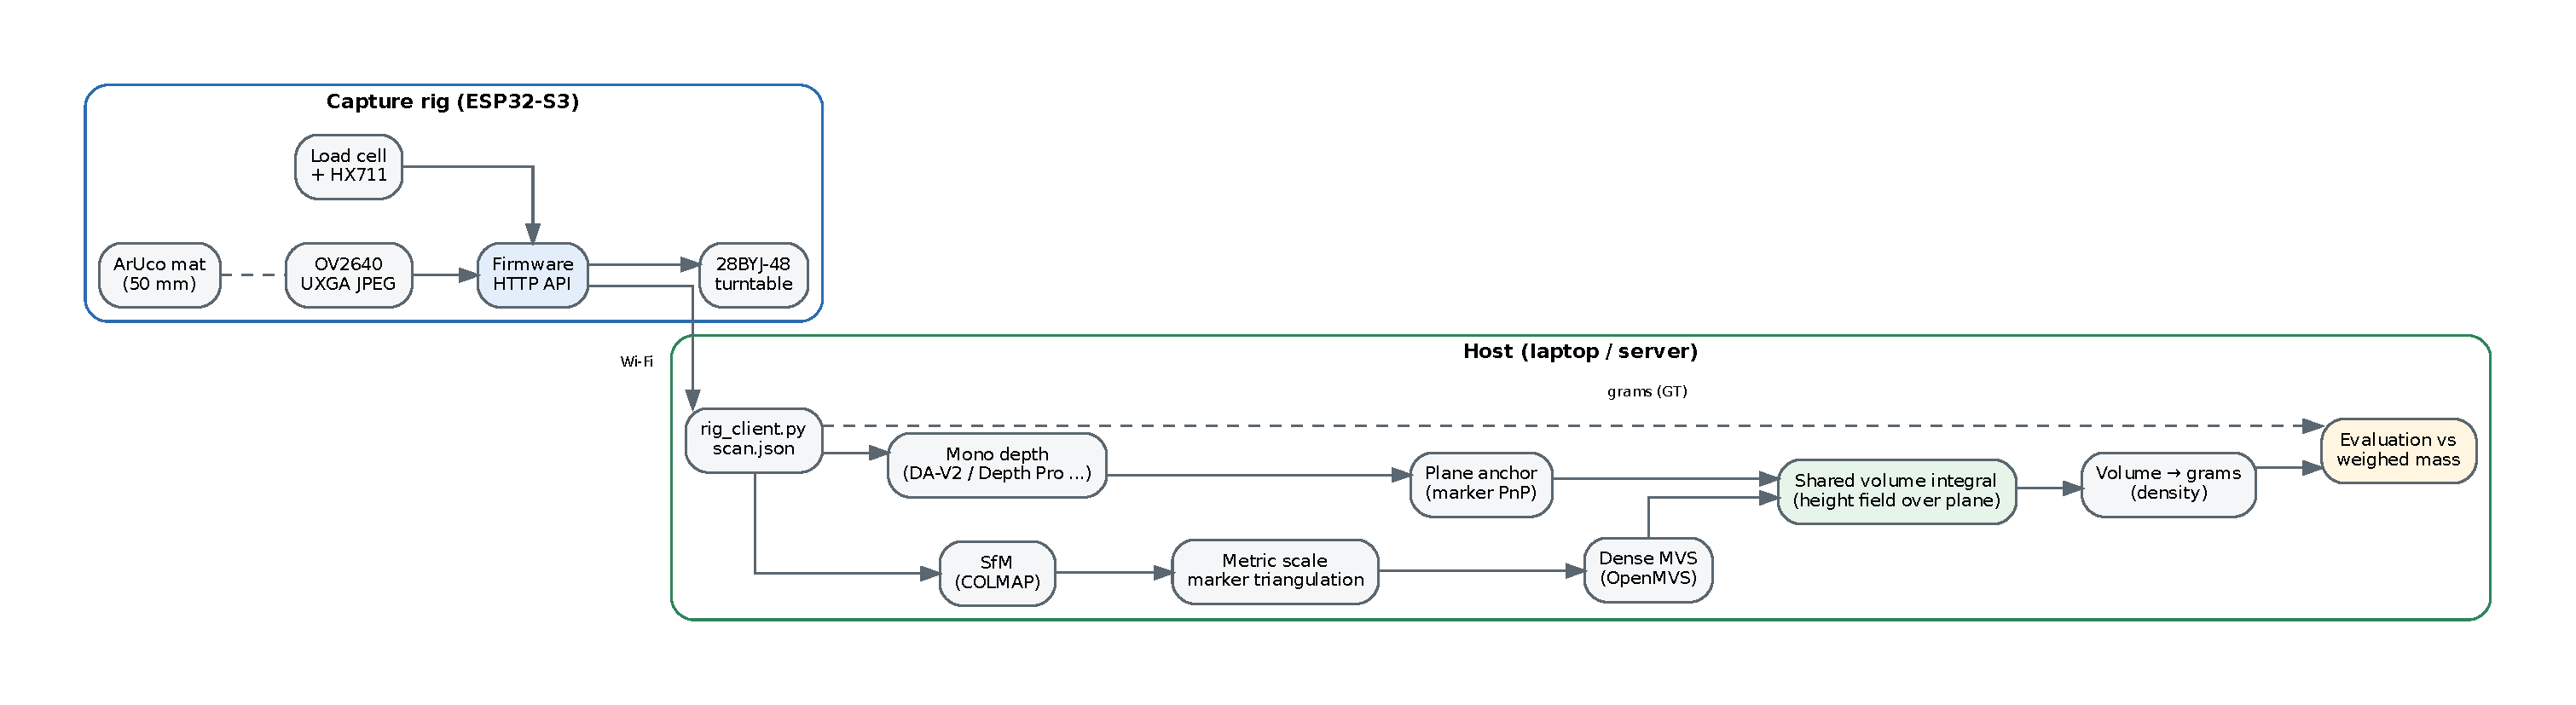
\includegraphics[width=\columnwidth]{figs/architecture.pdf}
\caption{System architecture. The rig exposes an HTTP API; the host drives the
scan loop, so dropped frames are retried rather than corrupting a scan.}
\label{fig:arch}
\end{figure}
\begin{figure}[t]\centering
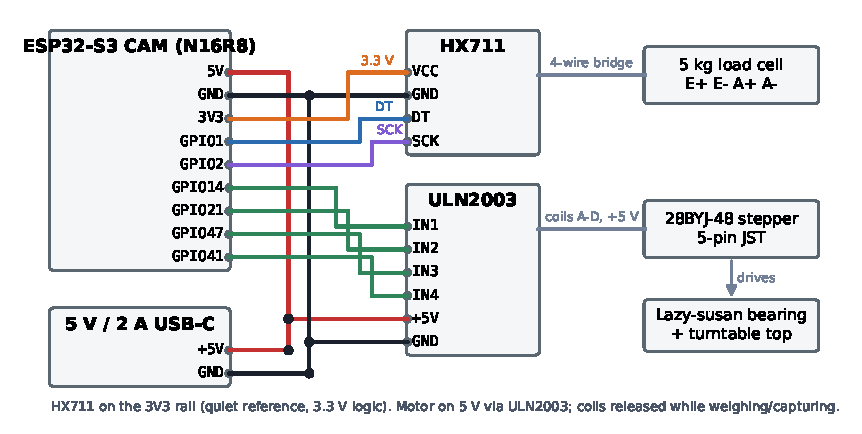
\includegraphics[width=\columnwidth]{figs/wiring.pdf}
\caption{Wiring of the ESP32-S3, HX711 load-cell amplifier and ULN2003 stepper driver.}
\label{fig:wiring}
\end{figure}
The rig (Fig.~\ref{fig:arch}, \ref{fig:wiring}) uses an ESP32-S3 camera board
(OV2640, up to $1600\times1200$), a 28BYJ-48 stepper through a ULN2003 driver
(4076 half-steps per revolution, \SI{0.088}{\degree} per step), and a
\SI{5}{kg} bar load cell read by an HX711 at 10\,Hz. The firmware exposes
\texttt{/capture}, \texttt{/rotate}, \texttt{/weight}, \texttt{/tare},
\texttt{/calibrate} and camera-setting endpoints. Exposure, gain and white
balance are locked after convergence so that all views of a scan share
photometry, which MVS assumes. Stepper coils are released while weighing to
avoid heating and vibration of the load cell. Tare and the counts-per-gram
calibration persist in flash. The firmware compiles for the ESP32-S3 target with
the Arduino core 3.3.12; a fake-firmware test exercises every client endpoint,
retry on a dropped frame, and calibration arithmetic.

\textbf{Physical validation (pending).} Load-cell linearity, repeatability and
drift, turntable angular error, scan duration and transfer latency are
specified as scripted bench tests (\texttt{rig\_client.py bench-*}) whose
results are \pending{to be measured on the assembled rig}. We report no
physical number we have not measured.

\section{Method}
\subsection{Shared volume integral}
All methods produce a 3-D point set $P$ in metres and a support plane
$(\mathbf n, d)$. Points are projected into an orthonormal plane basis, binned
into square cells, and each cell keeps the median (dense MVS) or the
back-projected height $h=\mathbf n^\top\mathbf p+d$. Empty cells inside the
footprint are filled by nearest neighbour, negative heights are clipped, and
$V=\sum_{\text{cells}} h\,c^2$. Because every method shares this integral,
differences in volume reflect differences in geometry.

\subsection{Metric scale from the marker mat}\label{sec:scale}
Marker corners are detected in every view and triangulated with the SfM
cameras; the scale $s$ is the ratio of the known side to the median
triangulated side. A relative error $\epsilon$ in $s$ produces a volume error of
$(1+\epsilon)^3-1\approx3\epsilon$, so a 1\,\% scale error costs about 3\,\% in
volume; Sec.~\ref{sec:synth} measures this directly.

\subsection{Monocular protocols}\label{sec:anchor}
\textbf{Raw}: the model's metric output is used as-is. \textbf{Anchor}: the
prediction is calibrated using only the support plane (the table in
Nutrition5k, the marker mat in our rig), never the food; metric outputs get one
scale, relative outputs an affine map of inverse depth. \textbf{Oracle}: the
same maps fitted to ground-truth depth over the whole dish region---an upper
bound that is not available at deployment. For relative models we record the
condition number of the anchor fit; a fronto-parallel plane has nearly
constant inverse depth, so scale and shift are not separately identifiable.

\section{Experiments}
\subsection{E1: Monocular depth on Nutrition5k}
\pending{e1 results}


\subsection{E2: Volume versus weighed mass}
Nutrition5k has no food-volume label, so the volume target in E1/E2 is the
volume integrated from RealSense depth over the dish region with the same
height-field integral (Eq.~\ref{eq:vol}) applied to each model's prediction.
The error therefore isolates the depth model: a model with zero error here
reproduces the sensor, whatever the sensor's own error on food is.
\pending{E2 table}



\subsection{E3: Multi-view versus monocular on exact synthetic volumes}\label{sec:synth}
\textbf{Scenes.} We specify twenty-two Blender (Cycles) scenes with watertight food meshes
whose volume is computed exactly from the mesh: eight food configurations
(single rice mound, rice + dal, two idli, curry heap, lumpy rice, a three-item
thali, a 40\,mL small portion and a tall mound) on ceramic and polished steel
plates (16 scenes), four textureless-food variants of the first four
configurations on ceramic, and two configurations on banana leaf. All 22 were
rendered and reconstructed. Each scene is rendered
at $1600\times1200$, $60^\circ$ horizontal FoV, $45^\circ$ elevation and
\SI{0.40}{m} distance, with the plate rotating on a turntable inside a printed
50\,mm ArUco mat, i.e.\ the rig geometry. View 0 also stores a metric depth map for a ``perfect single-view depth''
baseline.

\textbf{Methods.} We compare two pipelines. Dense MVS runs COLMAP SfM, takes
scale from the triangulated marker corners, densifies with OpenMVS, cuts the
food footprint at a threshold set from plate noise, and integrates. Sparse
SfM skips densification and integrates the SfM points with the same scale.
Single-view runs on these scenes are in the code but were not run, so the
monocular comparison rests on E1.

\textbf{Footprint rule.} Dense MVS leaves millimetre-level noise on the plate
surface. A cell counts as food if its height exceeds $\mu+2\sigma$ of the plate
annulus heights. This rule was fixed on \texttt{rice\_mound\_\_ceramic} before
the other scenes were run, and those scenes are held out. A hysteresis variant
(seed at $2\sigma$, grow connected cells down to $0.5\sigma$) was added
\emph{after} the curry failure below, and is reported as post hoc.

\begin{table*}[t]
\centering
\caption{E3 on synthetic plates with exact mesh volume. Error columns give the
median absolute error with a 95\% bootstrap CI across scenes; bias is the mean
signed error. Time: CPU seconds per scene on our VM.}
\label{tab:synth}
\footnotesize
\IfFileExists{tables/synth_main.tex}{\begin{tabular}{llrlrrr}\toprule
Method & Plate & $n$ ok & |err| \% median [95\% CI] & bias \% & $<$10\% & s \\
\midrule
MVS dense (24 views) & all & 11/11 & 3.9 [1.0, 5.7] & -4.0 & 10 & 117 \\
MVS dense (24 views) & ceramic & 6/6 & 5.3 [1.9, 16.0] & -5.7 & 5 & 114 \\
MVS dense (24 views) & steel & 5/5 & 2.0 [0.2, 4.2] & -1.9 & 5 & 119 \\
MVS dense, hysteresis (post-hoc) & all & 11/11 & 2.0 [0.3, 6.0] & +4.4 & 9 & 117 \\
MVS dense, hysteresis (post-hoc) & ceramic & 6/6 & 5.5 [1.7, 21.1] & +8.3 & 4 & 114 \\
MVS dense, hysteresis (post-hoc) & steel & 5/5 & 0.3 [0.1, 2.0] & -0.2 & 5 & 119 \\
\bottomrule
\end{tabular}
}{\pending{table}}
\end{table*}
\pending{E3 findings}



\subsection{E4: Ablations}
The ablations change one factor at a time and use the dense MVS pipeline,
except the marker-scale ablation, which used sparse SfM:
number of views (6, 8, 12, 16, 24, evenly spaced), image resolution
(1600$\times$1200, 800$\times$600, 640$\times$480, the OV2640 UXGA, SVGA and
VGA modes), JPEG re-encoding with OpenCV at quality 30 and 10 on its 0--100
scale (this is not the OV2640 0--63 quality register, and we did not measure
how the two map), a deliberate error in the printed marker size
($\pm1$, $\pm2\,\%$), plate material, and three repeated runs on identical
input to measure the run-to-run spread of SfM/MVS, which are not
bit-deterministic. A run fails if SfM returns no model, if no marker side is
triangulated, or if densification errors; failures are counted, not dropped.
The driver (\texttt{experiments/synth/run\_suite.py}) and the analysis
script are in the repository.
\textbf{Marker-scale error (60 runs, sparse SfM).} We scaled the believed marker
side by $0.98$--$1.02$ on 12 scenes. The recovered metric scale tracks the
injected factor, but the integrated volume does not change monotonically
(mean 71.7, 90.3, 77.9, 66.9 and 47.7\,mL for factors 0.98 to 1.02). Two sparse
runs of the same input differ by a median of 1.9 and up to 62.9 percentage
points of true volume, so run-to-run SfM variation is far larger than the
$\pm6\,\%$ that the cube law predicts for a $\pm2\,\%$ scale error. The cube law
is therefore an analytic bound (Sec.~\ref{sec:scale}), and this ablation is
uninformative on sparse reconstructions. It will be repeated on dense
reconstructions.

\textbf{View count (60 dense runs, 12 scenes).} Accuracy collapses below 12
views. The median absolute volume error is 91.6\,\% [78.7, 96.3] at 6 views
and 71.4\,\% [22.7, 76.5] at 8 views (0 and 2 of 12 scenes within 10\,\%). It
is 3.3\,\% [0.4, 19.2] at 12, 1.6\,\% [0.4, 3.6] at 16 and 4.2\,\% [0.4, 5.6]
at 24 views (9, 11 and 12 of 12 within 10\,\%). The paired difference between
16 and 24 views is not significant ($p=0.38$, Wilcoxon, $n=12$). Every view
registered at every setting; what drops is dense coverage (median 0.17\,M points
at 6 views against 1.03\,M at 24). Four idli runs at 6 and 8 views return fewer
than 1{,}000 food points and $-100\,\%$ volume while reporting success, so the
pipeline needs a minimum-food-point check before a scan is accepted. We keep 24
views as the default because it is the only setting with all scenes within
10\,\%; 16 views is the fallback when scan time matters. These runs were split
across three identical cloud VMs (8-vCPU Xeon, same package versions). The
pipeline is not bit-reproducible: the same 24-view input reconstructed on two
machines differed by a median of 0.9 percentage points, 10 of 12 scenes within
1.2 points, but by 4.9 points on \texttt{thali3\_\_ceramic} and 26.1 points on
\texttt{curry\_heap\_\_ceramic} ($-26.0\,\%$ vs.\ $+0.1\,\%$).

\textbf{Resolution and compression (72 dense runs, 12 scenes).} Resolution
matters less than compression. Median absolute volume error is 3.9\,\% [0.8,
5.1] at 1600$\times$1200 lossless and 3.2\,\% [2.1, 4.0] at 800$\times$600
lossless (12 of 12 within 10\,\%; paired $p=0.27$). OpenCV quality 30 at full
resolution is 7.4\,\% [2.4, 8.6] (12 of 12 within 10\,\%, $p=0.18$). Quality 10
fails at every resolution: 72.7\,\% at 1600$\times$1200, 90.4\,\% at
800$\times$600 and 82.7\,\% at 640$\times$480 (at most 1 of 12 within 10\,\%;
$p=4.9\times10^{-4}$ for each against the lossless baseline, significant after
Holm correction over five comparisons). Heavy compression removes the fine
texture that dense matching needs. For the rig this means a low compression
setting on the camera matters more than its maximum resolution; we did not
measure how the OV2640 quality register maps onto these OpenCV levels, so the
rig default has to be checked on hardware.

\textbf{Repeat runs (18 dense runs, 6 scenes, one machine).} Three runs on
identical input stay within 0.2--0.9 percentage points of each other on steel
plates and within 1.8--2.9 points on ceramic. The spread is again larger on the
textureless plate.

\textbf{Status.} Plate material beyond ceramic and steel (banana leaf) and
textureless food had not finished at the time of writing. Two observations are already available
from E3. Ceramic and steel differ in plate noise by about $2$--$5\times$
(plate-material ablation). Two independent reconstructions of the same eight
scenes differed by up to 2.7 percentage points (e.g.\ \texttt{idli\_pair\_\_ceramic}
$-8.4$ vs $-5.7$\,\%), which bounds run-to-run repeatability before the formal
repeat experiment.



\section{Limitations}
\textbf{Nutrition5k has no volume ground truth.} The dataset provides
overhead RealSense depth and weighed mass, not food volume. We therefore score
monocular models against the volume integrated from sensor depth over the same
dish region (food plus plate rim above the support plane). This measures how
well a model reproduces a depth sensor, not how well it measures food. Our
attempt to separate food from plate with a second plate-floor plane fit gave a
food volume that barely tracks weighed mass (Spearman $\rho=0.24$,
Pearson $r=-0.01$, $n=502$), so we do not use it as a target. Absolute food-volume
accuracy is reported only on synthetic scenes with exact mesh volume.

\textbf{Synthetic-to-real gap.} Blender scenes have perfect camera intrinsics,
controlled lighting and procedural textures. Real OV2640 frames add rolling
shutter, auto-exposure drift, lens distortion and JPEG blocking on low-texture
food. The resolution and JPEG ablations bound part of this gap but not all of it. Textureless food already fails in simulation (Sec.~\ref{sec:synth}); an active texture projector or image-space segmentation would be needed for it.

\textbf{No physical measurements yet.} Load-cell linearity, repeatability and
drift, turntable angular error, scan duration and Wi-Fi transfer latency have
scripts and empty tables (Sec.~\ref{sec:hw}); none of the numbers in this paper
come from the physical rig. Timings are CPU timings on 8-vCPU cloud VMs, not
on the ESP32-S3.

\textbf{Volume is not mass.} Converting volume to grams needs a per-food
density. We do not estimate density; the load cell measures mass directly, which
is the reason it is part of the rig.


\section{Conclusion}
We built a capture rig within an INR~5{,}000 budget and a
benchmark that scores monocular and multi-view volume estimation with the same
integral, explicit calibration protocols and confidence intervals. On the
partial results, three findings stand. First, a single overhead image
anchored only on the table does not recover food volume: the best deployable
model (ZoeDepth-NYU) still has a median error of 44\,\%, and relative models
lose almost all of it. Second, low depth error (AbsRel) does not imply low volume error.
Third, 24-view dense MVS with marker scale reaches a median error of a few
percent on exact synthetic volumes, its remaining error on textured food comes from
food--plate segmentation, and it fails on textureless food. Volume from depth does not predict grams on real
mixed dishes, which justifies the load cell. Next we will complete the remaining model
and scene runs, add image-space food segmentation, and run the physical
bench tests and real-plate captures.


\section*{Reproducibility}
All code, scene specifications, per-dish result files and the scripts that
generate every table and figure are in the repository. Evidence categories are
labelled throughout: \emph{Nutrition5k} (public real RGB-D data),
\emph{synthetic} (Blender/Cycles renders with exact mesh volume), \emph{VM}
(timings on an 8-core CPU-only cloud VM, not on the ESP32), and
\emph{physical} (pending rig measurements).

\bibliographystyle{IEEEtran}
\bibliography{refs}
\end{document}
